%!TEX root = cscw2019-comic.tex
\section{Results}
\label{sec:Study on Behavior Results}

In this section, we will first present the raw data used in the analysis, then introduce the Bayesian Model we used for data analysis and our analysis result.

\subsection{Raw Data}
\label{sub:Study on Behavior Raw Data}
In total, we have 307 participants joined our study, 101 participants received the message in the text form, 102 participants received the same message in the abstract comic form, and 104 participants received the abstract comic message with social-proof. We ran an outlier analysis using Tukey Fence on participants' completion time and removed 30 participants from our dataset. The following analysis is based on a dataset with 277 participants, 91 of them is in pure-text condition, 97 of them is in comic condition, and 92 of them is in comic-social-proof condition. Of those 277 participants, 150 were self-identified as male, and 126 were self-identified as female, 1 participant chose not to disclose. 197 participants earned at least college degree. The median annual household income of our study participants is \$50,000 - \$59,999.  All participants were familiar with the Autism Spectrum Disorder and acknowledged the importance of autism research. 

~\Cref{fig:contributions across conditions} compares the distributions of the charitable donations across the three conditions. Among all 307 participants, 253 (82.4\%) participants donated non-zero amount to support the autism research; 74 (73.3\%) participants from the text condition, 86 (84.3\%) participants from the comic condition, and 93 (89.4\%) participants from the comic with social proof condition.


\begin{figure*}[htb]
	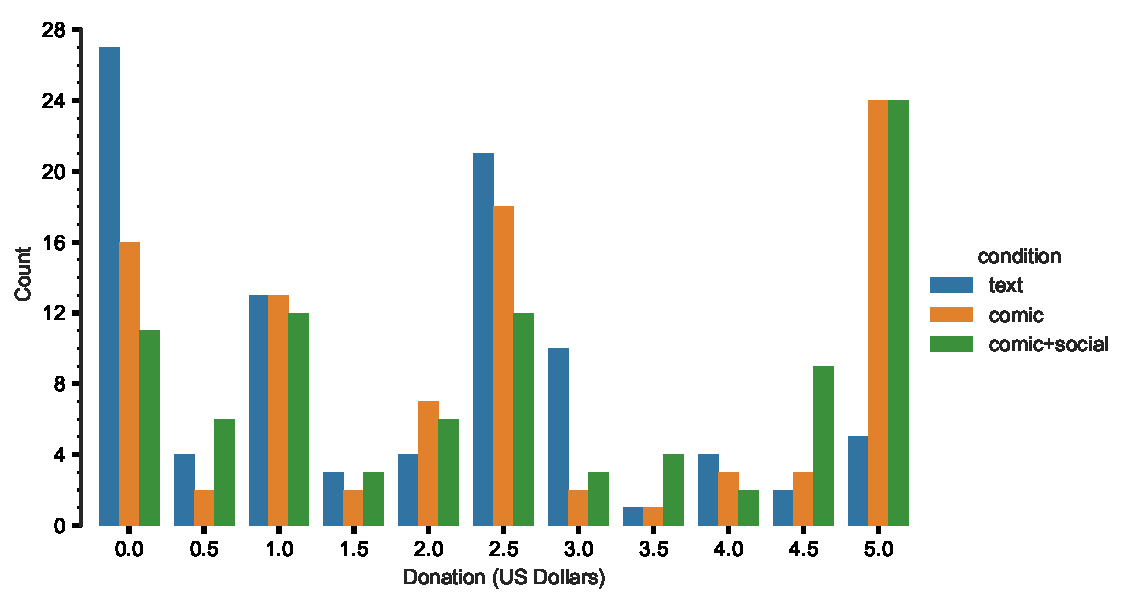
\includegraphics[width=1\textwidth]{./hari-code/contributions_across_conditions.pdf}
    \caption{The distribution of the amount of money participants decide to donate to the charity in each of the three conditions: text only; comic; comic with social proof. Among all 307 participants, 253 (82.4\%) participants donated non-zero amount to support the autism research; 74 (73.3\%) participants from the text condition, 86 (84.3\%) participants from the comic condition, and 93 (89.4\%) participants from the comic with social proof condition.
}
	\label{fig:contributions across conditions}
\end{figure*}

% \begin{figure*}[htb]
% 	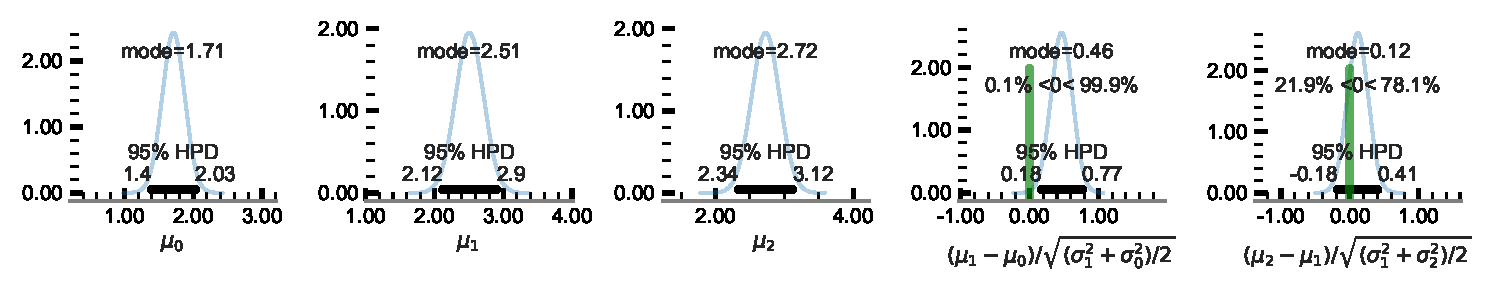
\includegraphics[width=1\textwidth]{./hari-code/new_exp_text_v_comic_v_social.pdf}
%     \caption{The posterior distribution of the amount of money participants decide to donate to the charity in each of the three conditions: text only ($\mu_0$); comic ($\mu_1$); comic with social norm ($\mu_2$). The right two panels are respectively: posterior distribution of the effect size contrasting the comic condition ($\mu_1$) and text ($\mu_0$); the effect size contrasting comic with social norm ($\mu_2$) with the plain comic ($\mu_1$). First notice that $\mu_2 > \mu_1 > \mu_0$. Furthermore, the modal effect size of comparing the comic panel against text is 0.48, a medium effect and the HPD interval $[0.17, 0.77]$ reliably excludes a ROPE of $[0 \pm 0.1]$, indicating that the effect is meaningful. The effect of introducing the social norm into the comic has a minor effect (mode=0.12) when contrasted against the plan comic, and the HPD interval $[-0.17, 0.41]$ includes a ROPE of $[0 \pm 0.1]$, indicating that the outcome is not convincing.}
% 	\label{fig:main-experiment2-effect}
% \end{figure*}
\subsection{Bayesian Formulation}
\label{sub:Bayesian Formulation}
We use a Bayesian formulation of the problem of identifying suitable predictors for the messages in comic form.~\textcite{Kay2016} provide a nice introduction on the appropriateness of Bayesian analysis for the HCI community. Bayesian analysis is attractive in our experiment due to two advantages: shifting the conversation from ``did it work'' to ``how strong is the effect''; and benefits to small $n$ studies. 

Our experiment has three experimental groups: text, comic and comic with the social proof. One way to use classical statistical analysis for multiple groups would be to use ANOVA to see if the treatment (the use of comic) has any effect.  Bayesian inference can sometimes differ from the standard ANOVA test widely used to compare treatment effects.


% This is because the $t$-test assumes that the two populations from which samples are drawn, follow a Normal distribution, an assumption that can be violated in practice. Non-Normality is easily accounted for in a Bayesian formulation and~\textcite[][p. 470]{Kruschke2014} points out that the Normality assumption is one explanation why a $t$-test may be less sensitive to differences than a Bayesian analysis.

This is because ANOVA assumes equal variances within groups, and that the response within each group is drawn from a Normal distribution---in practice, both assumptions may be violated.  It is straightforward in Bayesian Analysis to relax both assumptions: equal variances and Normality. The Normality assumption may be one reason why ANOVA and the $t$-test may be less sensitive to differences than Bayesian analysis~\parencite[][p. 470]{Kruschke2014}.

\begin{figure*}[htb]
	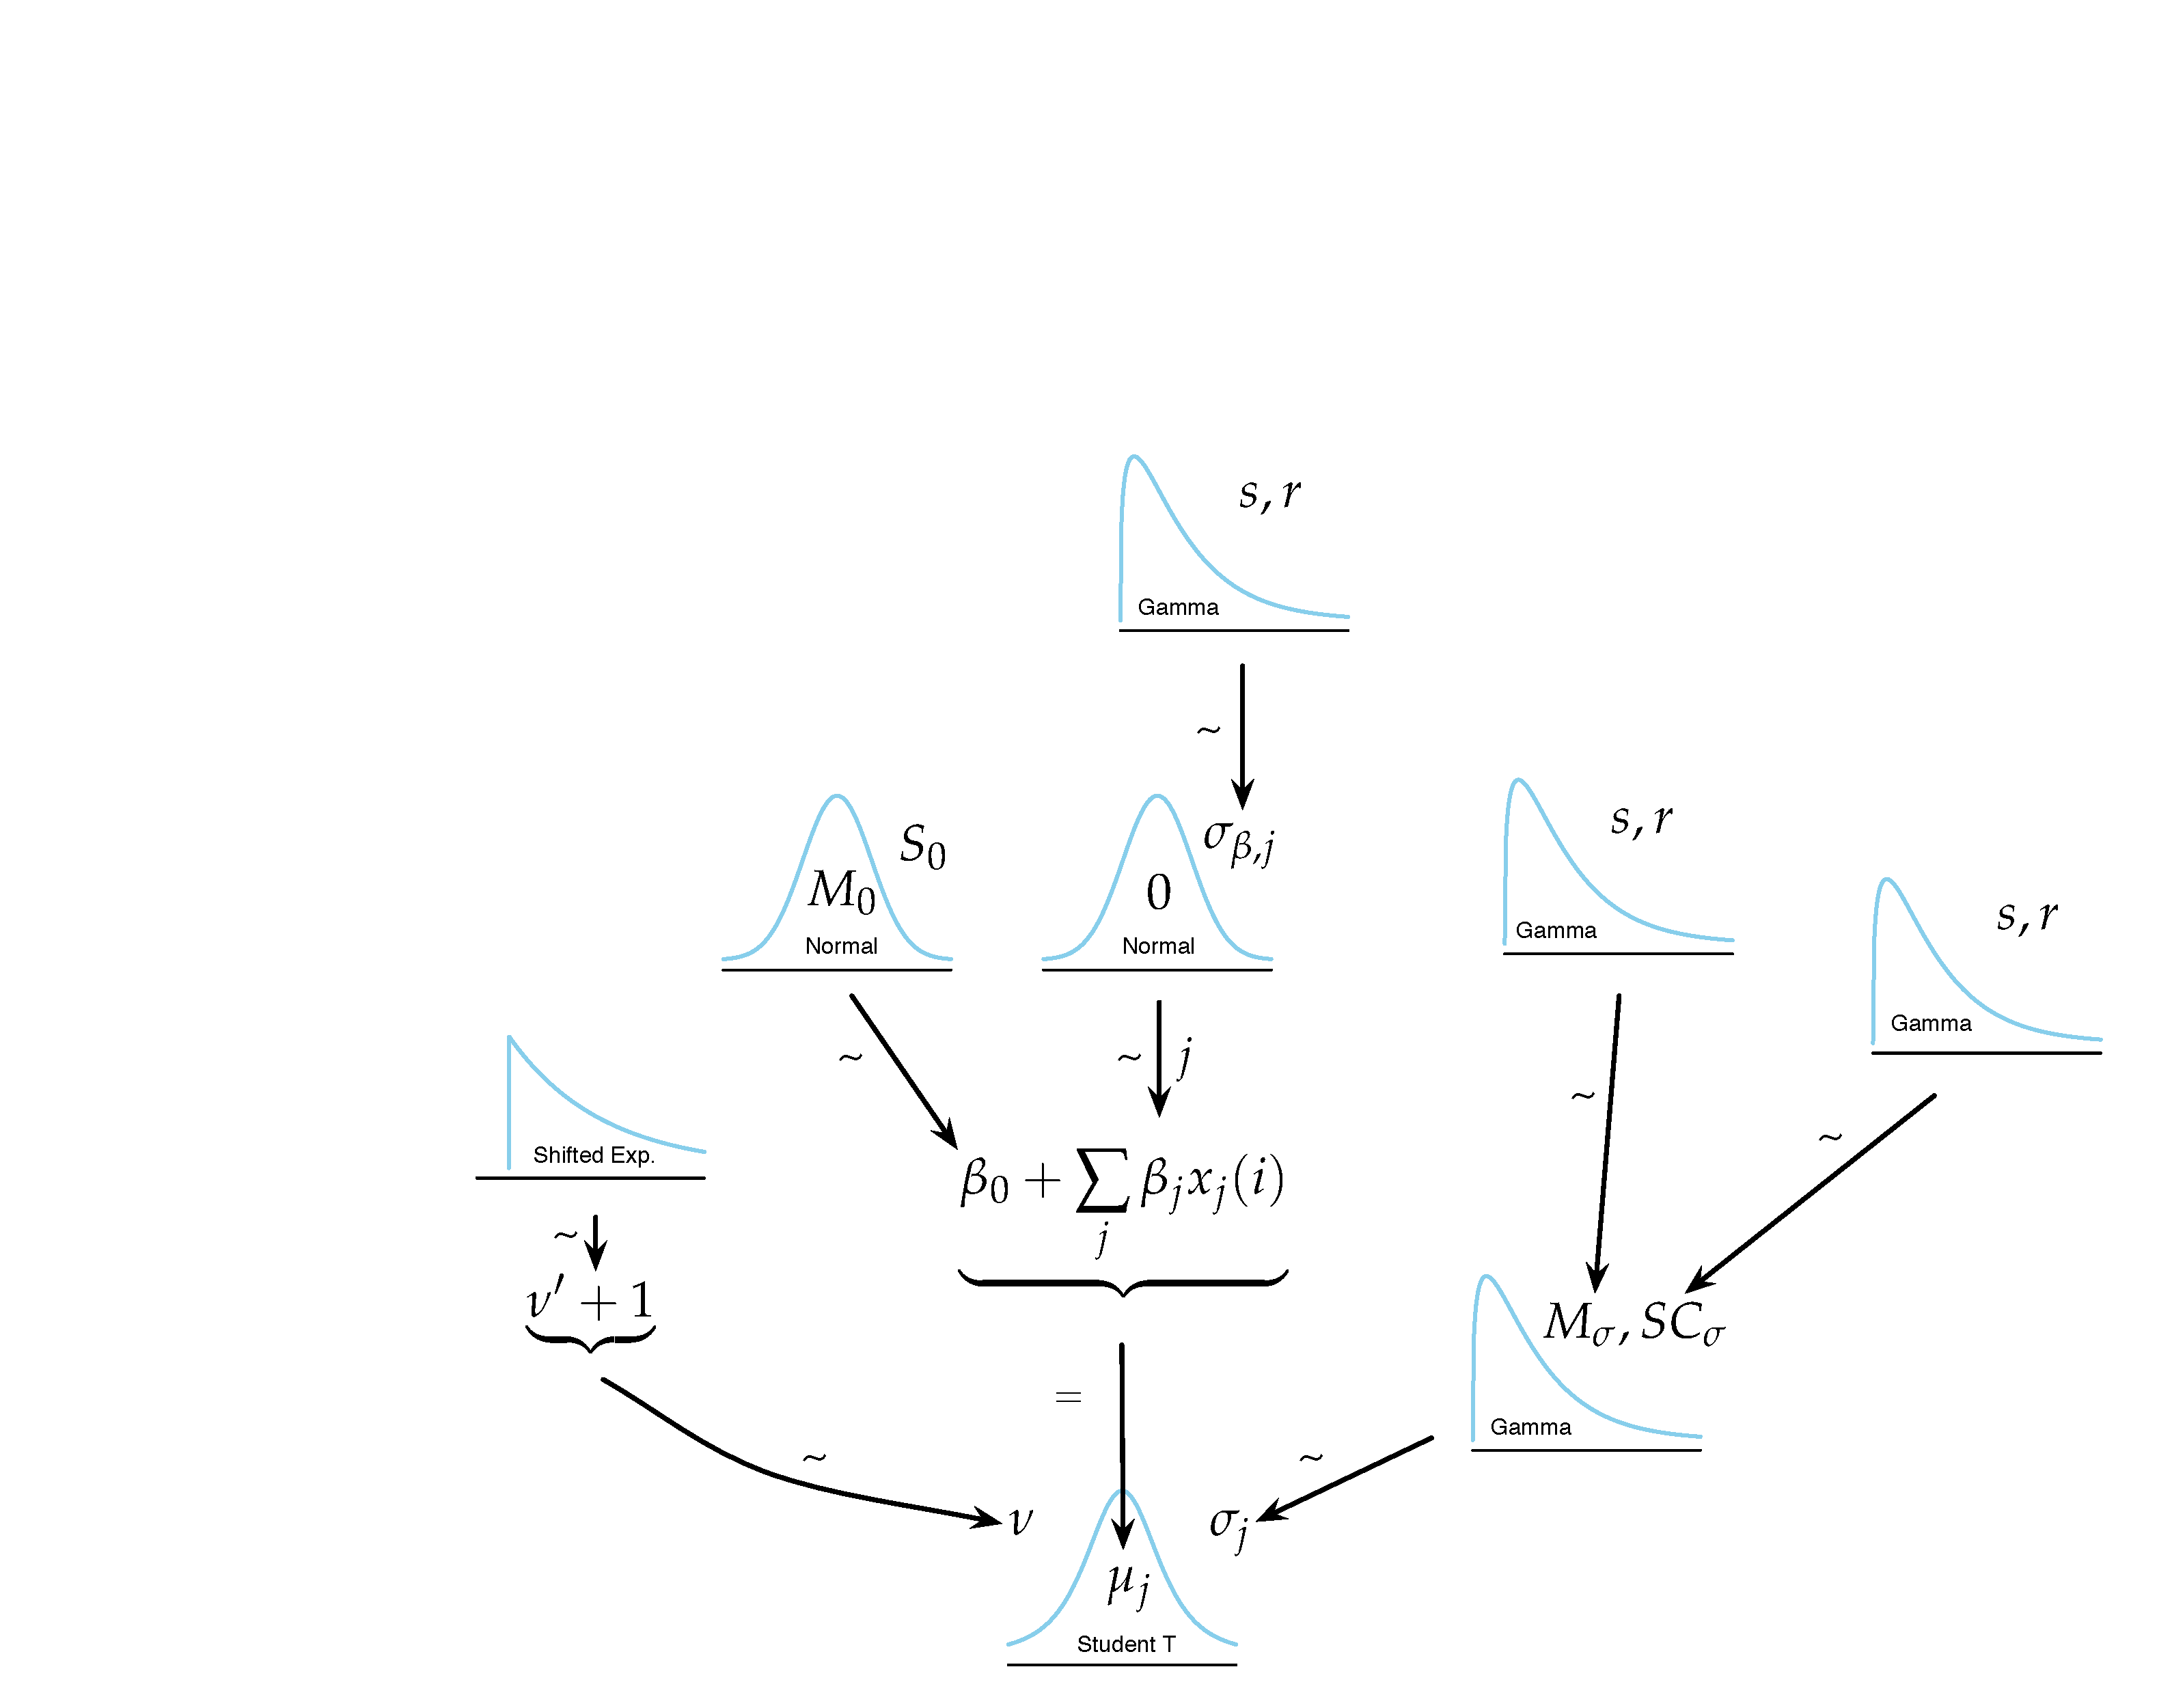
\includegraphics[width=1\textwidth]{./figures/gen_model.pdf}
    \caption{Our proposed Hierarchical Bayesian model.}
	\label{fig:generative model}
\end{figure*}



Now, we discuss our Bayesian formulation (see~\Cref{fig:generative model} for a graphical view of the model). There is one outcome variable $y_{i \mid j}$, the amount of donation to the charity by each participant $i$, under experimental condition $j$: text, comic, and comic with social proof. Our Bayesian model:


\begin{align}
    y_{i \mid j} \sim &  \mathrm{StudentT}(\nu, \mu_j, \sigma_j), \label{eq:bayesian formulation}\\
    \nu \sim & 1 + \exp(\lambda), \\
    \mu_j \sim & \beta_0 + \sum_j \beta_j x_j(i), \label{eq:mean response}\\
    \sigma_j \sim & \Gamma(M_{\sigma}, SC_{\sigma}),\\
    M_{\sigma} \sim & \Gamma(s,r), \\
    SC_{\sigma} \sim & \Gamma(s,r), \\
    \beta_0 \sim & N(M_0, SD_0), \\
    \beta_j \sim & N (0, \sigma_{\beta, j}), \\
    \sigma_{\beta, j} \sim & \Gamma(s,r).
\end{align}
 
\Cref{eq:bayesian formulation} says that the response $y_{i \mid j}$ of each group $j$ is modeled as a $\mathrm{StudentT}$ distribution with mode $\mu_j$,  scale $\sigma_j$ and with $\nu$ degrees of freedom; notice that this is a \textit{drawing distribution}, not the $t$-test. The $\mathrm{StudentT}$ allows us to model a non-Normal outcome with a heavy tail; assuming $y_{i \mid j}$ to be Normally distributed is equivalent to setting $\nu=\infty$. The degrees of freedom $\nu$ is drawn from a shifted exponential distribution, to ensure $\nu \geq 1$; the mode $\mu_j$ corresponding to each group is drawn from a Normal distribution with $\mu_j = \beta_0 + \sum_j \beta_j x_j(i)$, where the group indicator variable $x_j(i)=1 \iff \text{subject } i \text{ belongs to group } j$. The scale $\sigma_j$ of the normal distribution is drawn from a Gamma distribution $\Gamma(M_{\sigma}, SC_{\sigma})$, with mode $M_{\sigma}$ and scale $SC_{\sigma}$. The mode $M_{\sigma}$ and scale $SC_{\sigma}$ are each drawn from two independent Gamma distributions $\Gamma(s,r)$ with shape parameter $s$ and rate parameter $r$. The overall group response $\beta_0$ is modeled as a Normal distribution with mean $\mu_0$ and variance $\sigma_0$. For each of the $\beta_j$ for each group $j$ in~\Cref{eq:mean response}, $\beta_j$ is Normally distributed with mean $\mu=0$ and $\sigma_{\beta, j}$ drawn from a Gamma distribution $\Gamma(s,r)$ with shape parameter $s$ and rate parameter $r$. The random variables $\beta_j$ are centered around $\mu=0$ so that the group responses are modeled as deflections around the overall mean $\beta_0$. 

~\Cref{fig:generative model} indicates that we draw all the variances $\sigma_{\beta, j}$ from a Gamma $\Gamma(s,r)$ distribution, where $s$ refers to the shape parameter and $r$ refers to the rate parameter. We set the variables $s,r$ to allows a wide range of values for $\sigma_{\beta, j}$. Notice that we draw the variances $\sigma_{\beta, j}$ of each group $j$ independently from a \textit{common} Gamma distribution, implying that the variances (equivalently, the extent of deflections from the mean) for each predictor $\beta_j$ can be different. The main advantage of using a Gamma distribution is that we can specify a non-zero mode, important in controlling shrinkage in hierarchical models. 

We draw the scale variables $\sigma_{j}$ of the likelihood StudentT distribution from a common Gamma distribution, whose rate and shape parameters are also drawn from Gamma distributions. The advantage of this hierarchical approach is that the values of each element of $\sigma_j$ inform the other elements. The ``information sharing'' among variables common to hierarchical Bayesian models and is an important reason why Bayesian models work so well with small datasets\footnote{The sharing of information causes the scale of each group $\sigma_{j}$ to move towards the group variance, a phenomenon known as ``shrinkage.'' }. Finally, the constants $M_0, S_0, s, r$ are set so that the priors are generous but weakly informative so that despite exploring all possible values, we ensure rapid MCMC convergence.



% The result ~\Cref{fig:main-experiment2-effect} shows the modal effect size between abstract-comic v. pure-text = 0.48; There is no overlap of the 95\% high probability density (HPD) interval with the ROPE of [-0.1, 0.1]. Thus the effect is of medium size and meaningful; the effect size between abstract-comic and social-proof-comic is 0.12; but since the distribution includes a ROPE of $[-0.1 \pm 0.1]$, the effect is not convincing.

\subsection{Analysis}
\label{sub:Analysis}

We analyzed the data using PyMC3~\cite{Salvatier2016}, a popular framework for Bayesian inference. Computational techniques for Bayesian inference use a stochastic sampling technique called Markov Chain Monte Carlo (MCMC) that samples the posterior distribution $P(\theta | D)$, where we want to estimate the parameters $\theta$ given the observations $D$. In particular, we used the No-U Turn Sampler (NUTS) sampler. 

\begin{figure*}[htb]
	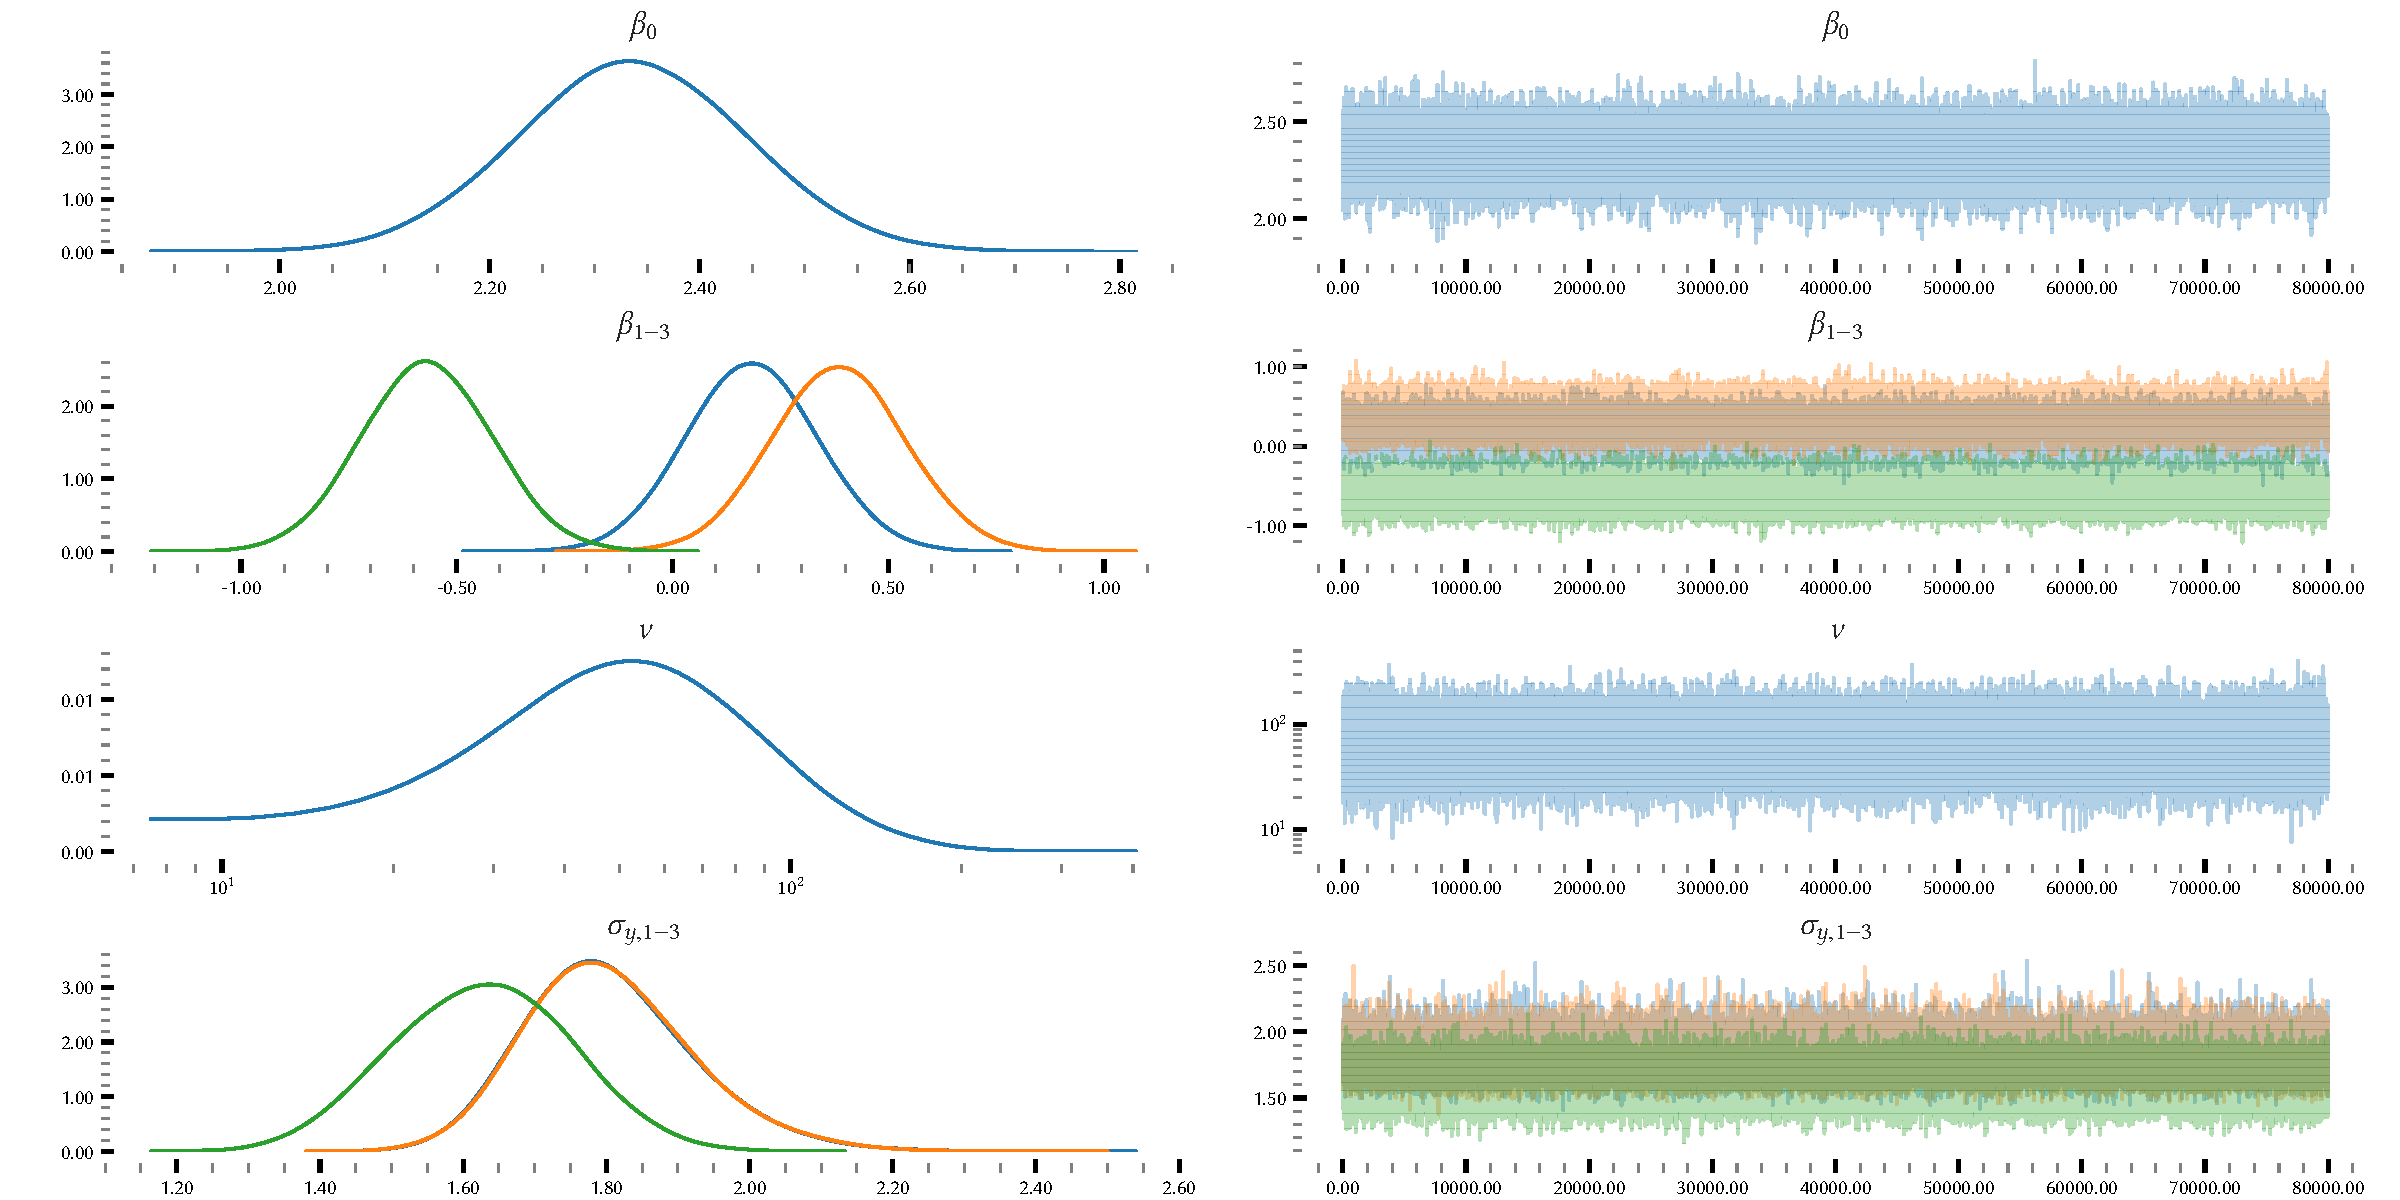
\includegraphics[width=1\textwidth]{./hari-code/robust_traceplot.pdf}
    \caption{Traceplot showing the results of the MCMC estimation. Left column shows the posterior distributions for $\beta_0, \beta_{[1-3]}, \mu_{[1-3]}, \nu, \sigma_{[1-3]}$, while the right column shows the corresponding traces. The posterior plots for $\nu$, the parameter corresponding to degrees of freedom has a modal value of $\nu=53$. While the ideal case of $\nu=\infty$ makes the StudentT distribution equivalent to the Normal distribution, in practice $\nu \geq 30$ is used to test for Normality. Thus the response distributions $y_{i \mid j}$ tend towards Normality. Notice that the mean of $\sigma_2$ (green curve, fourth panel, left column), variance of the group response in the case of text, is less than $\sigma_1$ or $\sigma_3$ (variances of the group responses for the comic, comic+social norm cases respectively), justifying our modeling assumptions of unequal variances across groups; the variances for the two comic conditions are nearly identical. The Gelman-Rubin statistic $\hat{R}$ was around 1, indicating that the different sampling chains converged. Furthermore, the effective sample size of all parameters was greater than 10,000. }
	\label{fig:traceplot}
\end{figure*}


 

Our analysis shows that the abstract comic form has a clear treatment effect over the corresponding text message.~\Cref{fig:robustcontrasts} shows the contrast and the effect size of the contract for four cases. The first three columns of~\Cref{fig:robustcontrasts} show the contrasts (top row) and the corresponding effect size (bottom row) between a pair of experimental conditions. The fourth column is a comparison between the text condition and the comic condition, by pooling together responses of the two comic conditions.

Let us examine one result (`text' v. `comic') in detail; the analysis for the other cases follows a similar logic. The top left sub-figure shows that the contrast has a mode of $0.75$ with the High Posterior Density (HPD\footnote{The HPD interval is the location of 95\% of the posterior density. This is similar to, but different from the idea of the confidence interval used in non-Bayesian Statistics. In non-Bayesian Statistics, a confidence interval of say 95\% is informally interpreted as ``with 95\% probability the parameter of interest lies in a specific interval; the tails are of equal width (i.e. 2.5\%)''; the HPD on the other hand, is the \textit{densest} interval covering 95\% of the posterior. The HPD is guaranteed to include the most likely value, but this is not always true for confidence intervals; see~\textcite[][p. 57]{McElreath2015} for a simple example. For a more careful definition of the confidence interval, see~\textcite{Hoekstra2014}, which also includes a discussion on the misinterpretation of confidence intervals.}) interval of $[0.26, 1.27]$. That is, subjects most frequently donate $\$0.75$ more on in the comic condition than in the text condition, with 95\% of the \textit{increase in donations} lying between $[\$0.26, \$1.27]$. Since the HPD lies outside a meaningful ROPE (Region of Practical Equivalence)\footnote{Unlike non-Bayesian Statistics, where one can ask for example, if the two means for two treatments are different $P(\mu_1\neq \mu_2)$, in Bayesian statistics, one asks if the HPD interval of the distribution $P(\mu_1-\mu_2)$, that is, the distribution of the difference of the means of the two treatments, excludes an interval where we can consider the two treatments equivalent. This equivalence interval is domain dependent. } of $0 \pm 0.1$, the result implies that there is a clear effect due to the treatment. Furthermore, the lower left sub-figure shows a moderate to medium effect size of $0.44$; we consider an effect of $0.2$ to be small, and an effect of $0.5$ is a medium-sized effect. Since the distribution excludes the ROPE interval $[0 \pm 0.1]$, half of the small-sized effect value of $0.2$, the discovered effect size is meaningful. 

The second column contrasts the comic with social proof case (`comic+social') with the plain text (`text'). We find that the contrast has a mode of $0.95$ with the High Posterior Density (HPD) interval of $[0.44, 1.47]$. The modal effect size is $0.55$, with an HPD interval of $[0.25, 0.86]$ which excludes a ROPE of $0 \pm 0.1$ indicating a meaningful, slightly larger than a medium-sized effect.

The third column contrasts the donations in the comic (`comic') condition against the comic with the social proof (`comic+social'). While the contrast is positive with a mode of $0.19$, notice that the HPD interval $[-0.31, 0.72]$ overlaps a ROPE of $0 \pm 0.1$ implying that the observed differences are not meaningful. The corresponding modal effect size of this contrast is $0.11$ with an HPD of $[-0.17, 0.39]$ with about 21.9\% of the HPD lying to the left of 0, implying that the observed effect size is not meaningful.


\begin{figure*}[htb]
	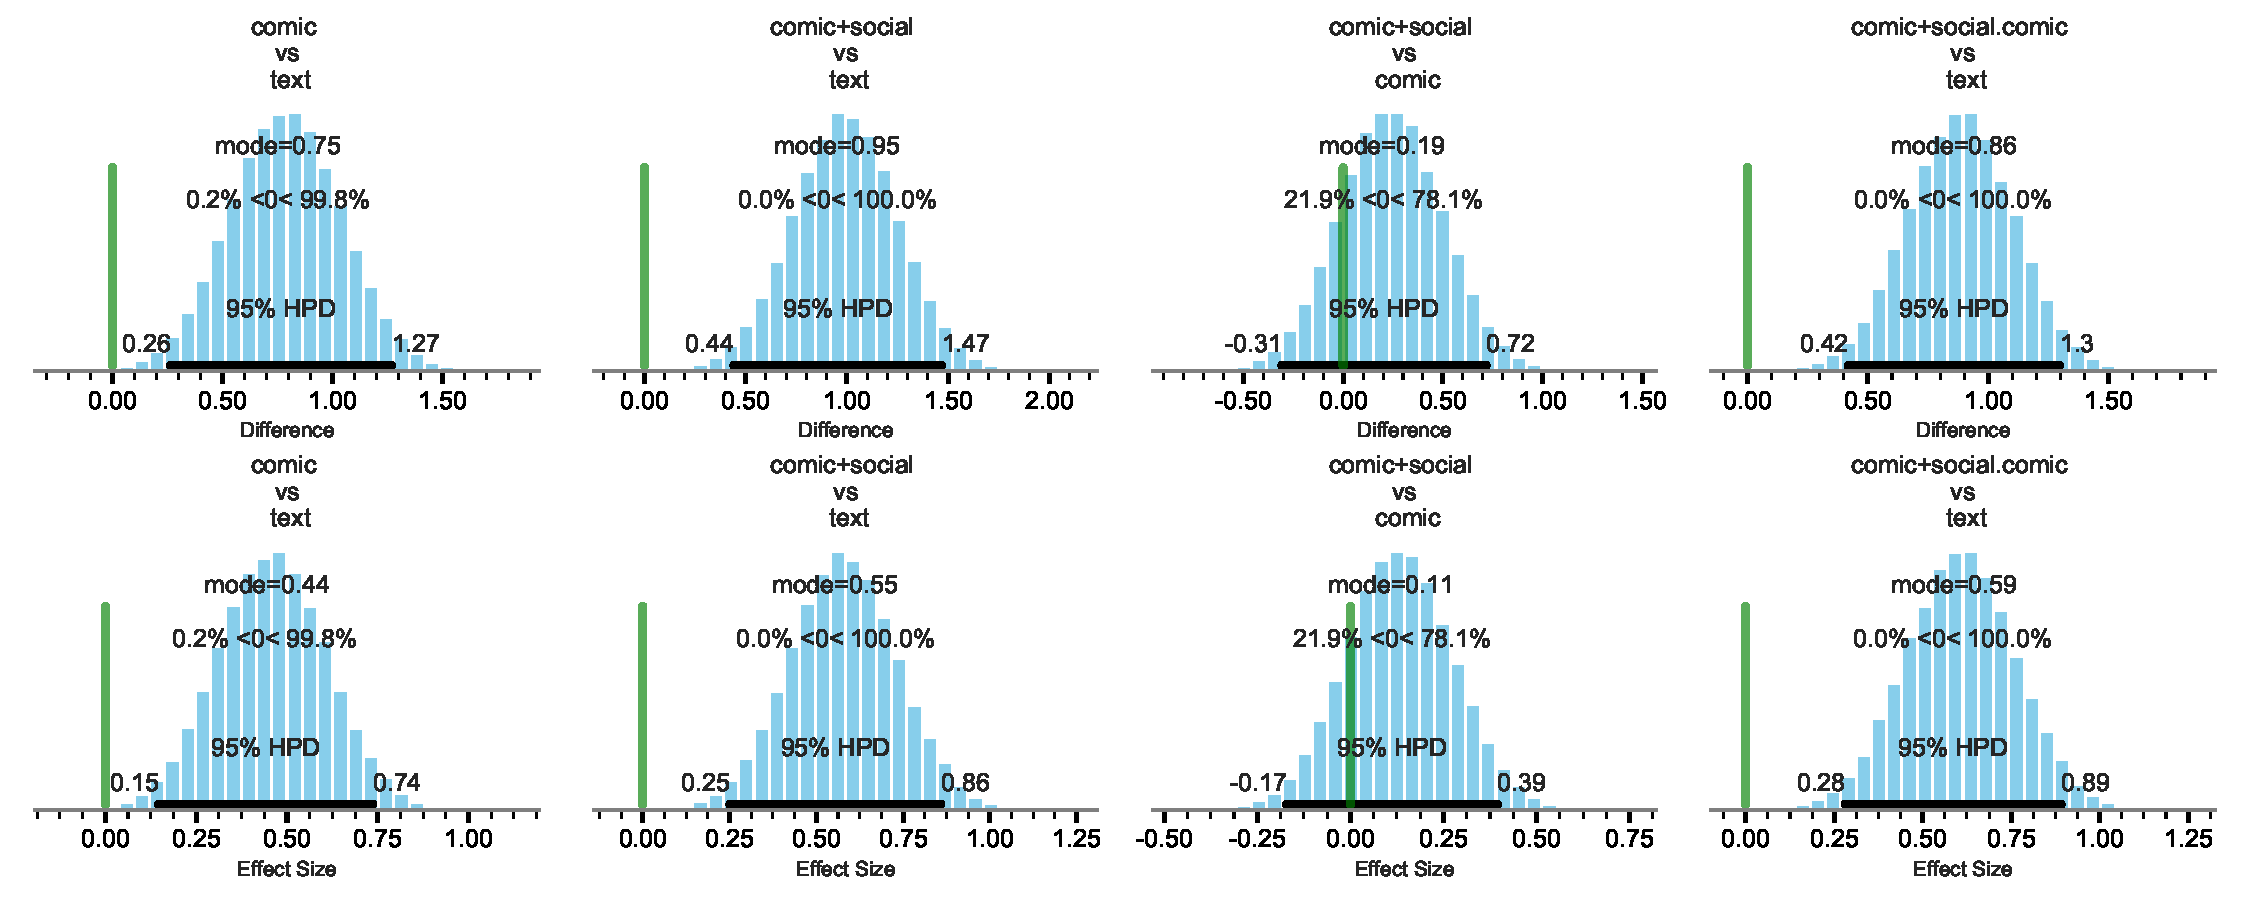
\includegraphics[width=1\textwidth]{./hari-code/robust_contrasts.pdf}
    \caption{The figure shows contrasts between the three experimental conditions (`text', `comic', `comic+social'). We also show in the fourth column contrasts between the text condition and pooled case of the two comic conditions to highlight the effect of using the abstract comic. Since we are highlighting contrasts, each sub-figure also shows a green line located at 0.The main finding: the comic treatment creates a medium to large sized effect (mode=0.59, pooled case, fourth column, bottom) when compared to the `text' condition. There is a slight increase in effect size when using the comic with social proof (`comic+social', second column, bottom) in comparison to the case when there is a comic without the social proof (`comic', first column, bottom). However, these differences are not meaningful, since the about 21.2\% of the HPD of the contrast between the `comic' and the `comic+social' case lies to the left of 0.0 (second column). }
	\label{fig:robustcontrasts}
\end{figure*}

The fourth column of~\Cref{fig:robustcontrasts} compares the text condition (`text') with the comic condition by pooling the responses in the two comic conditions. The pooling of the `comic' and the `comic+social' data is straightforward in Bayesian analysis. Since the MCMC \textit{jointly} estimates the posteriors of all variables, we can create a new variable that averages the values of the posteriors of the `comic' and `comic+social' cases for every step of the MCMC, to represent an averaged 'comic' condition.  We find that the contrast has a mode of $0.86$ with the High Posterior Density (HPD) interval of $[0.42, 1.30]$. Notice that the HPD interval is narrower than the corresponding HPD intervals comparing (`text' v. `comic' ) and (`text' v. `comic+social') The modal effect size is $0.59$, with an HPD interval of $[0.28, 0.89]$ which excludes a ROPE of $0 \pm 0.1$ indicating a meaningful, a medium to large sized effect, where the large effect size is $0.8$. 

In this section, we presented a Bayesian model to analyze the overall effect of using an abstract-comic to persuade people making charitable donation decisions, and understand the effect of adopting persuasive techniques in the abstract comic form. The results show that the use of abstract-comic produces a meaningful, medium to large modal effect ($0.59$) in persuading participants to donate. Although abstract-comic with social proof (`comic+social') can produce a larger effect that the case without social proof (`comic'), the contrast between abstract-comic and abstract-comic with social proof is not meaningful. The code and data will be released after publication. Next, we discuss the findings, design implications and limitations.
